\documentclass{article}
\usepackage{enumitem}
\usepackage[document]{ragged2e}
\usepackage{tikz}
\usetikzlibrary{shapes,arrows}
\usetikzlibrary{positioning}
\tikzstyle{block} = [rectangle, draw, 
    text width=4in, text centered, minimum height=2em]
\tikzstyle{block2} = [rectangle, draw, 
    text width=2in, text centered, minimum height=2em]
\tikzstyle{line} = [draw, -latex']
\renewcommand{\labelitemi}{\labelitemii}
\renewcommand{\labelitemiii}{\labelitemii}
\usepackage{xcolor}
\usepackage{graphicx}
\usepackage{microtype}
\usepackage{amsmath}
\usepackage[paperwidth=30in,paperheight=36in,top=1in,bottom=1in,left=1in,right=1in]{geometry}
\usepackage{lipsum}
\usepackage{fontspec}
\usepackage{tikz}
\usetikzlibrary{matrix,chains,positioning,decorations.pathreplacing,arrows}

\setmainfont[SizeFeatures={{Size=-11,Color=red},
                           {Size=11-30,Color=blue},
                           {Size=30-,Color=green}}]{Univers LT Std}

% \renewcommand*{\familydefault}{\sfdefault}

% DIN 1451 Std or DIN 30640 Std for descriptions
% Trade Gothic LT for titles
\begin{document}
\begin{minipage}[c]{20in}
{ 
\fontspec{Trade Gothic LT}[Color=red]
\fontsize{4in}{0.8in}\selectfont 
% THE COOPER \\\hspace{-0.85in} UNION
% THE \vspace{0.2in}\\ COOPER UNION
\bfseries
WHO'S THAT \vspace{0in}\\ PLANKTON?
}
\end{minipage}
\vspace{1in}\\
\colorbox{white}{
\begin{minipage}{28in}
\centering
% \includegraphics[width=20in]{solmaris.jpg}
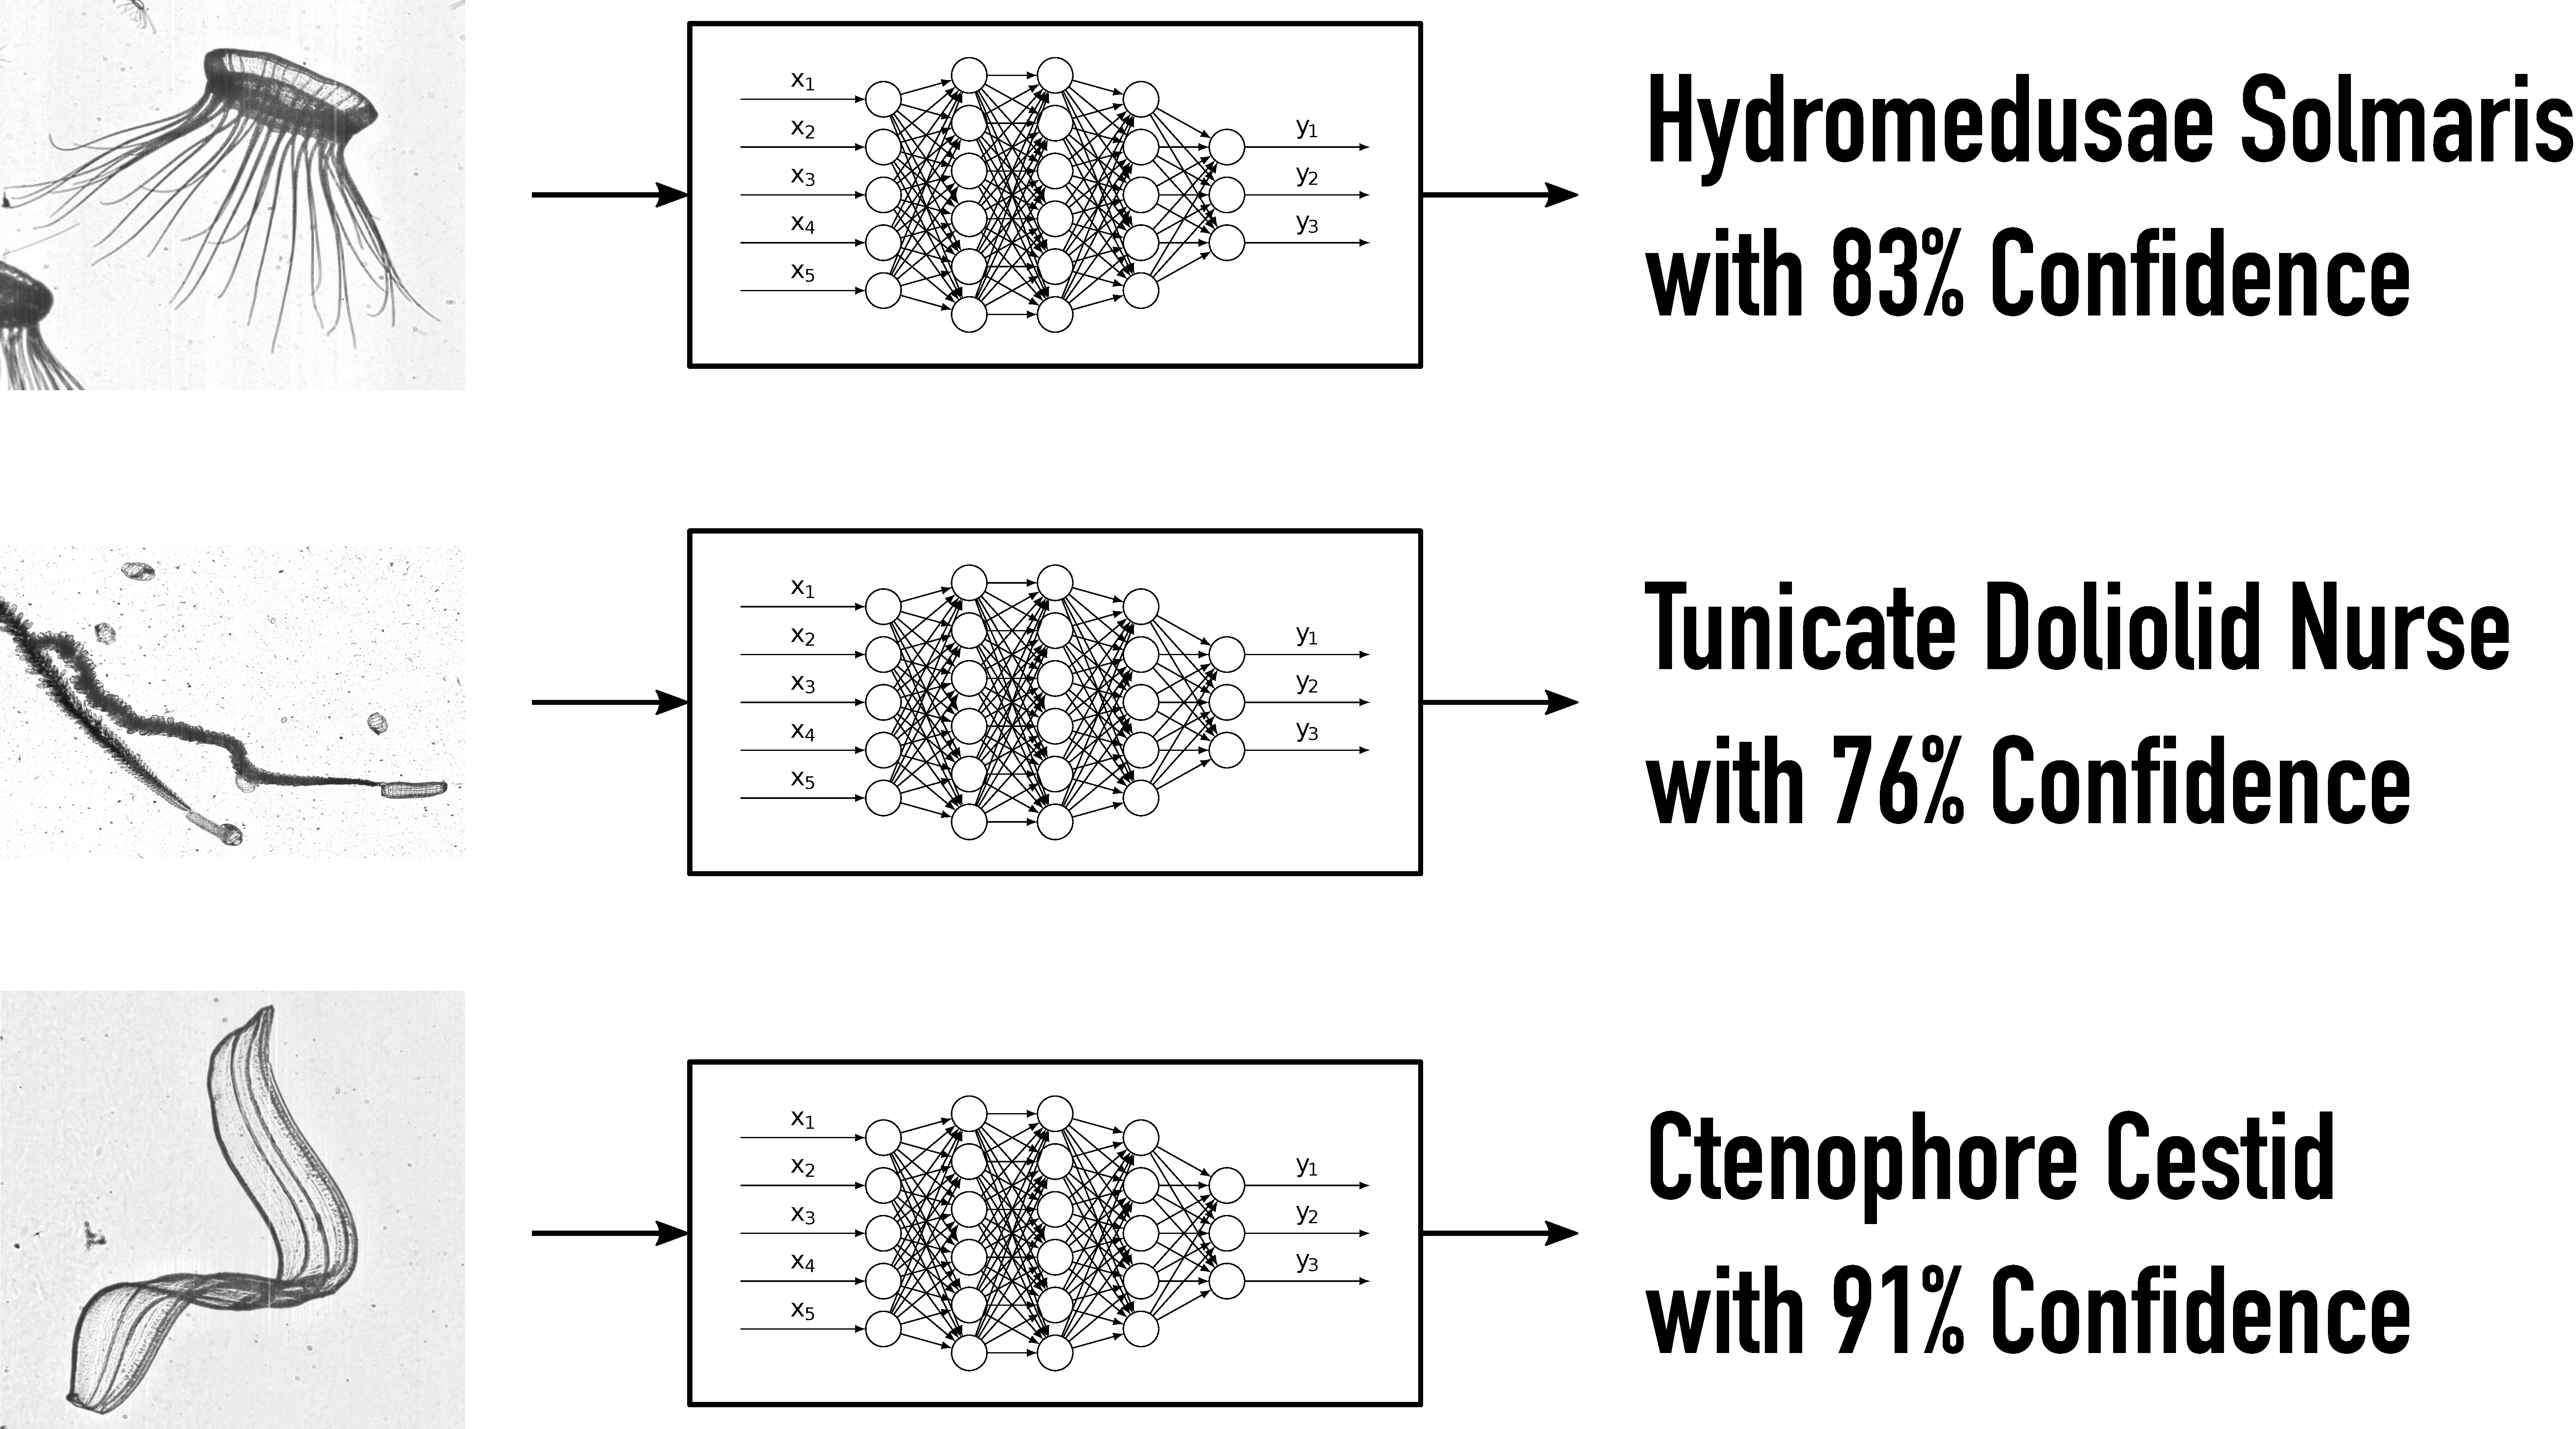
\includegraphics[width=25in]{figure.pdf}
% 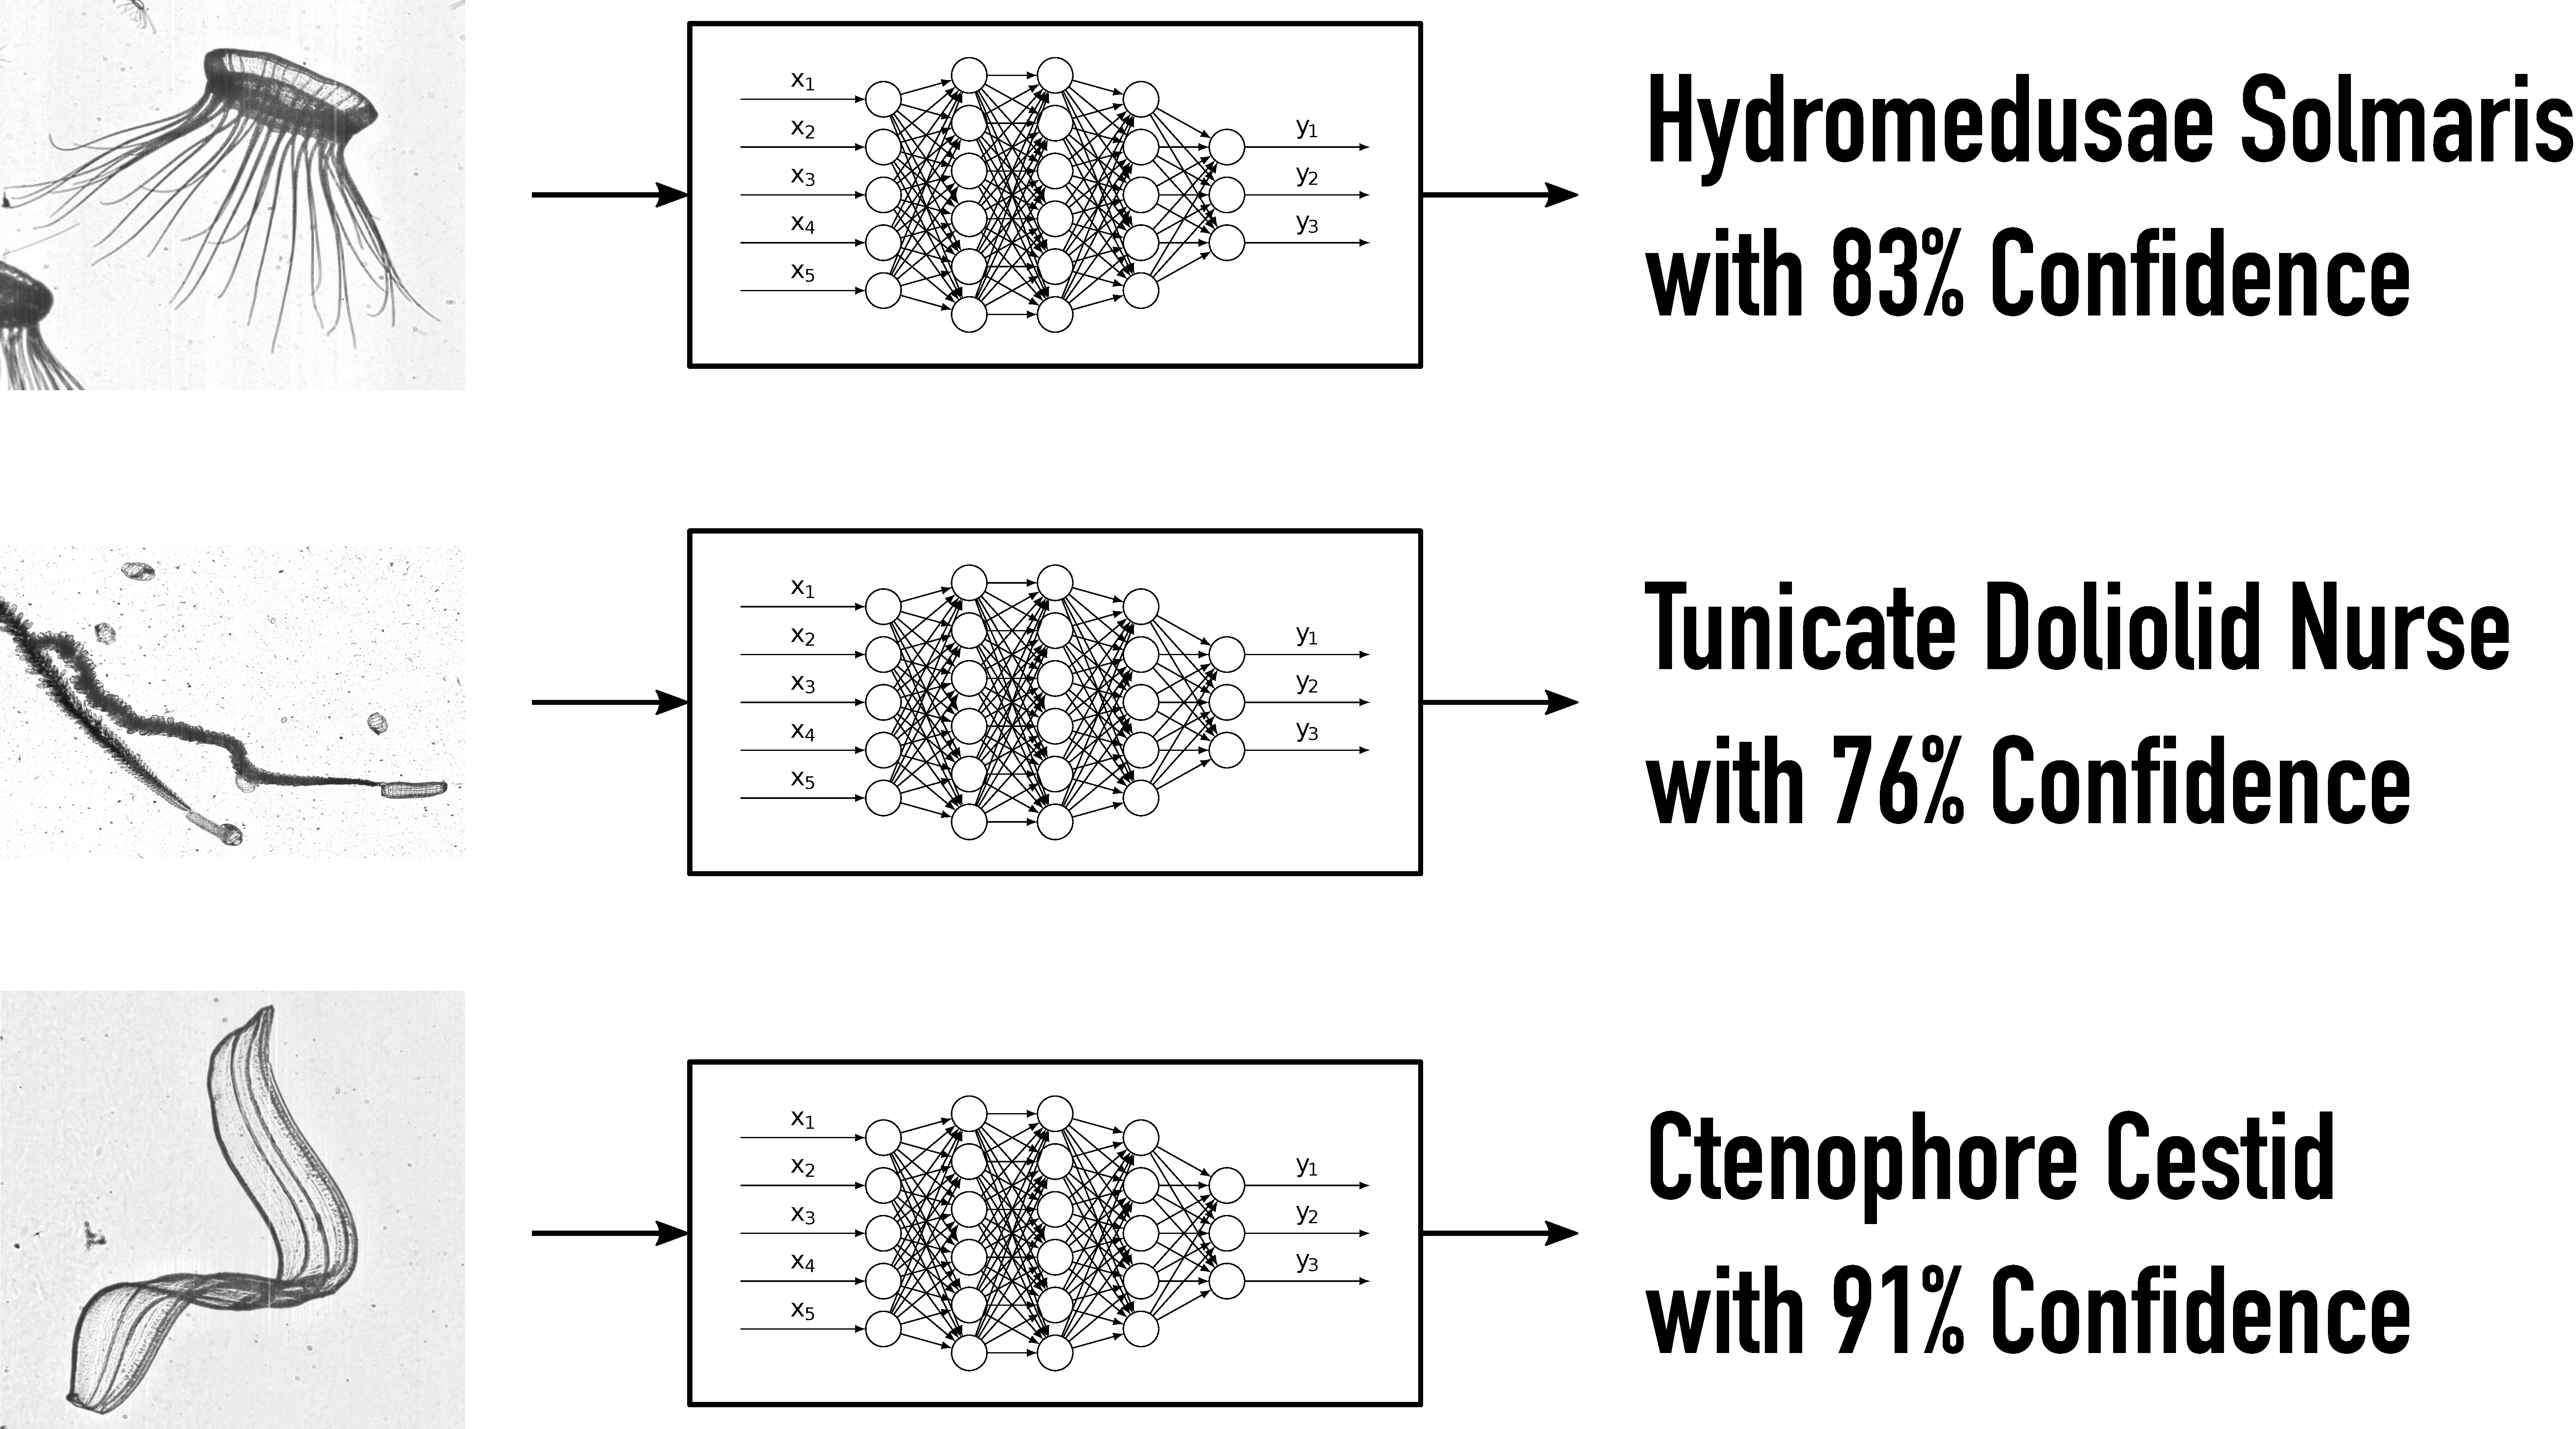
\includegraphics[scale=1]{figure.pdf}
% \includegraphics[width=0.7\linewidth]{fb.png}
\end{minipage}
}
\vspace{1in}\\
{
\fontspec{DIN 1451 Std}[Color=black]
\fontsize{1in}{1em}\selectfont 
CHRIS CURRO
}
{
\fontspec{DIN 1451 Std}[Color=black]
\fontsize{0.8in}{1em}\selectfont 
EE '15 AND
}
{
\fontspec{DIN 1451 Std}[Color=black]
\fontsize{1in}{1em}\selectfont 
HARRISON ZHAO
}
{
\fontspec{DIN 1451 Std}[Color=black]
\fontsize{0.8in}{1em}\selectfont 
EE '16, ADVISOR: SAM KEENE
}
\vspace{0.8in}\\
\begin{minipage}{16.8in}
{
	% \fontspec{DIN 30640 Std}
	\fontspec{DIN 1451 Std}[Color=black]
	\fontsize{0.6in}{8em}\selectfont

    We created a system for the automatic classification of different species
	of plankton. We utilize convolutional neural networks and the Torch 7 framework
	to create powerful statistical models that determine plankton species directly from
	images like the ones above. We created the system to compete in the National Data Science Bowl, 
	where we placed 29$^\text{th}$ (97$^\text{th}$ percentile) in the world and were one of the
	top student teams.


} \end{minipage} 
\hfill
\begin{minipage}{11in}
{
	% \fontspec{DIN 30640 Std}
	\fontspec{DIN 1451 Std}[Color=black]
	\fontsize{0.6in}{8em}\selectfont
	\begin{tabbing}
	Source Code: \= github.com/harrisonzhao/plankton \\
	More Info: \> ee.cooper.edu/\textasciitilde{}curro/plankton.pdf
	\end{tabbing}
} \end{minipage} 
\end{document}

